% ============================================================================================
% BAB IV DESAIN KONSEP SOLUSI
% ============================================================================================

\chapter{DESAIN KONSEP SOLUSI}
\label{chap:desain-konsep}

Bagian setelah ini mengilustrasikan desain konsep solusi yang diusulkan dalam bentuk model konseptual. Model ini dirancang untuk dapat dibandingkan secara langsung ("before and after") dengan arsitektur sistem saat ini yang telah dianalisis pada Bab II.

\section{Desain Konsep Solusi yang Diusulkan (\textit{After})}
\label{sec:konsep_after}

Dalam upaya menjembatani kesenjangan tersebut, diusulkan suatu desain solusi
perangkat lunak yaitu, \textbf{Arsitektur Integrasi Dinamis} (atau "Model Umpan Balik Ganda"), sesuai dengan hasil analisis pada Subbab \ref{ssec:analisis_penentuan_solusi}. Model konseptual dari arsitektur solusi ini diilustrasikan pada Gambar \ref{fig:model-konseptual-solusi} dalam bentuk \textit{UML Activity Diagram}.

\begin{figure}[H]
    \centering
    \captionsetup{justification=centering}
    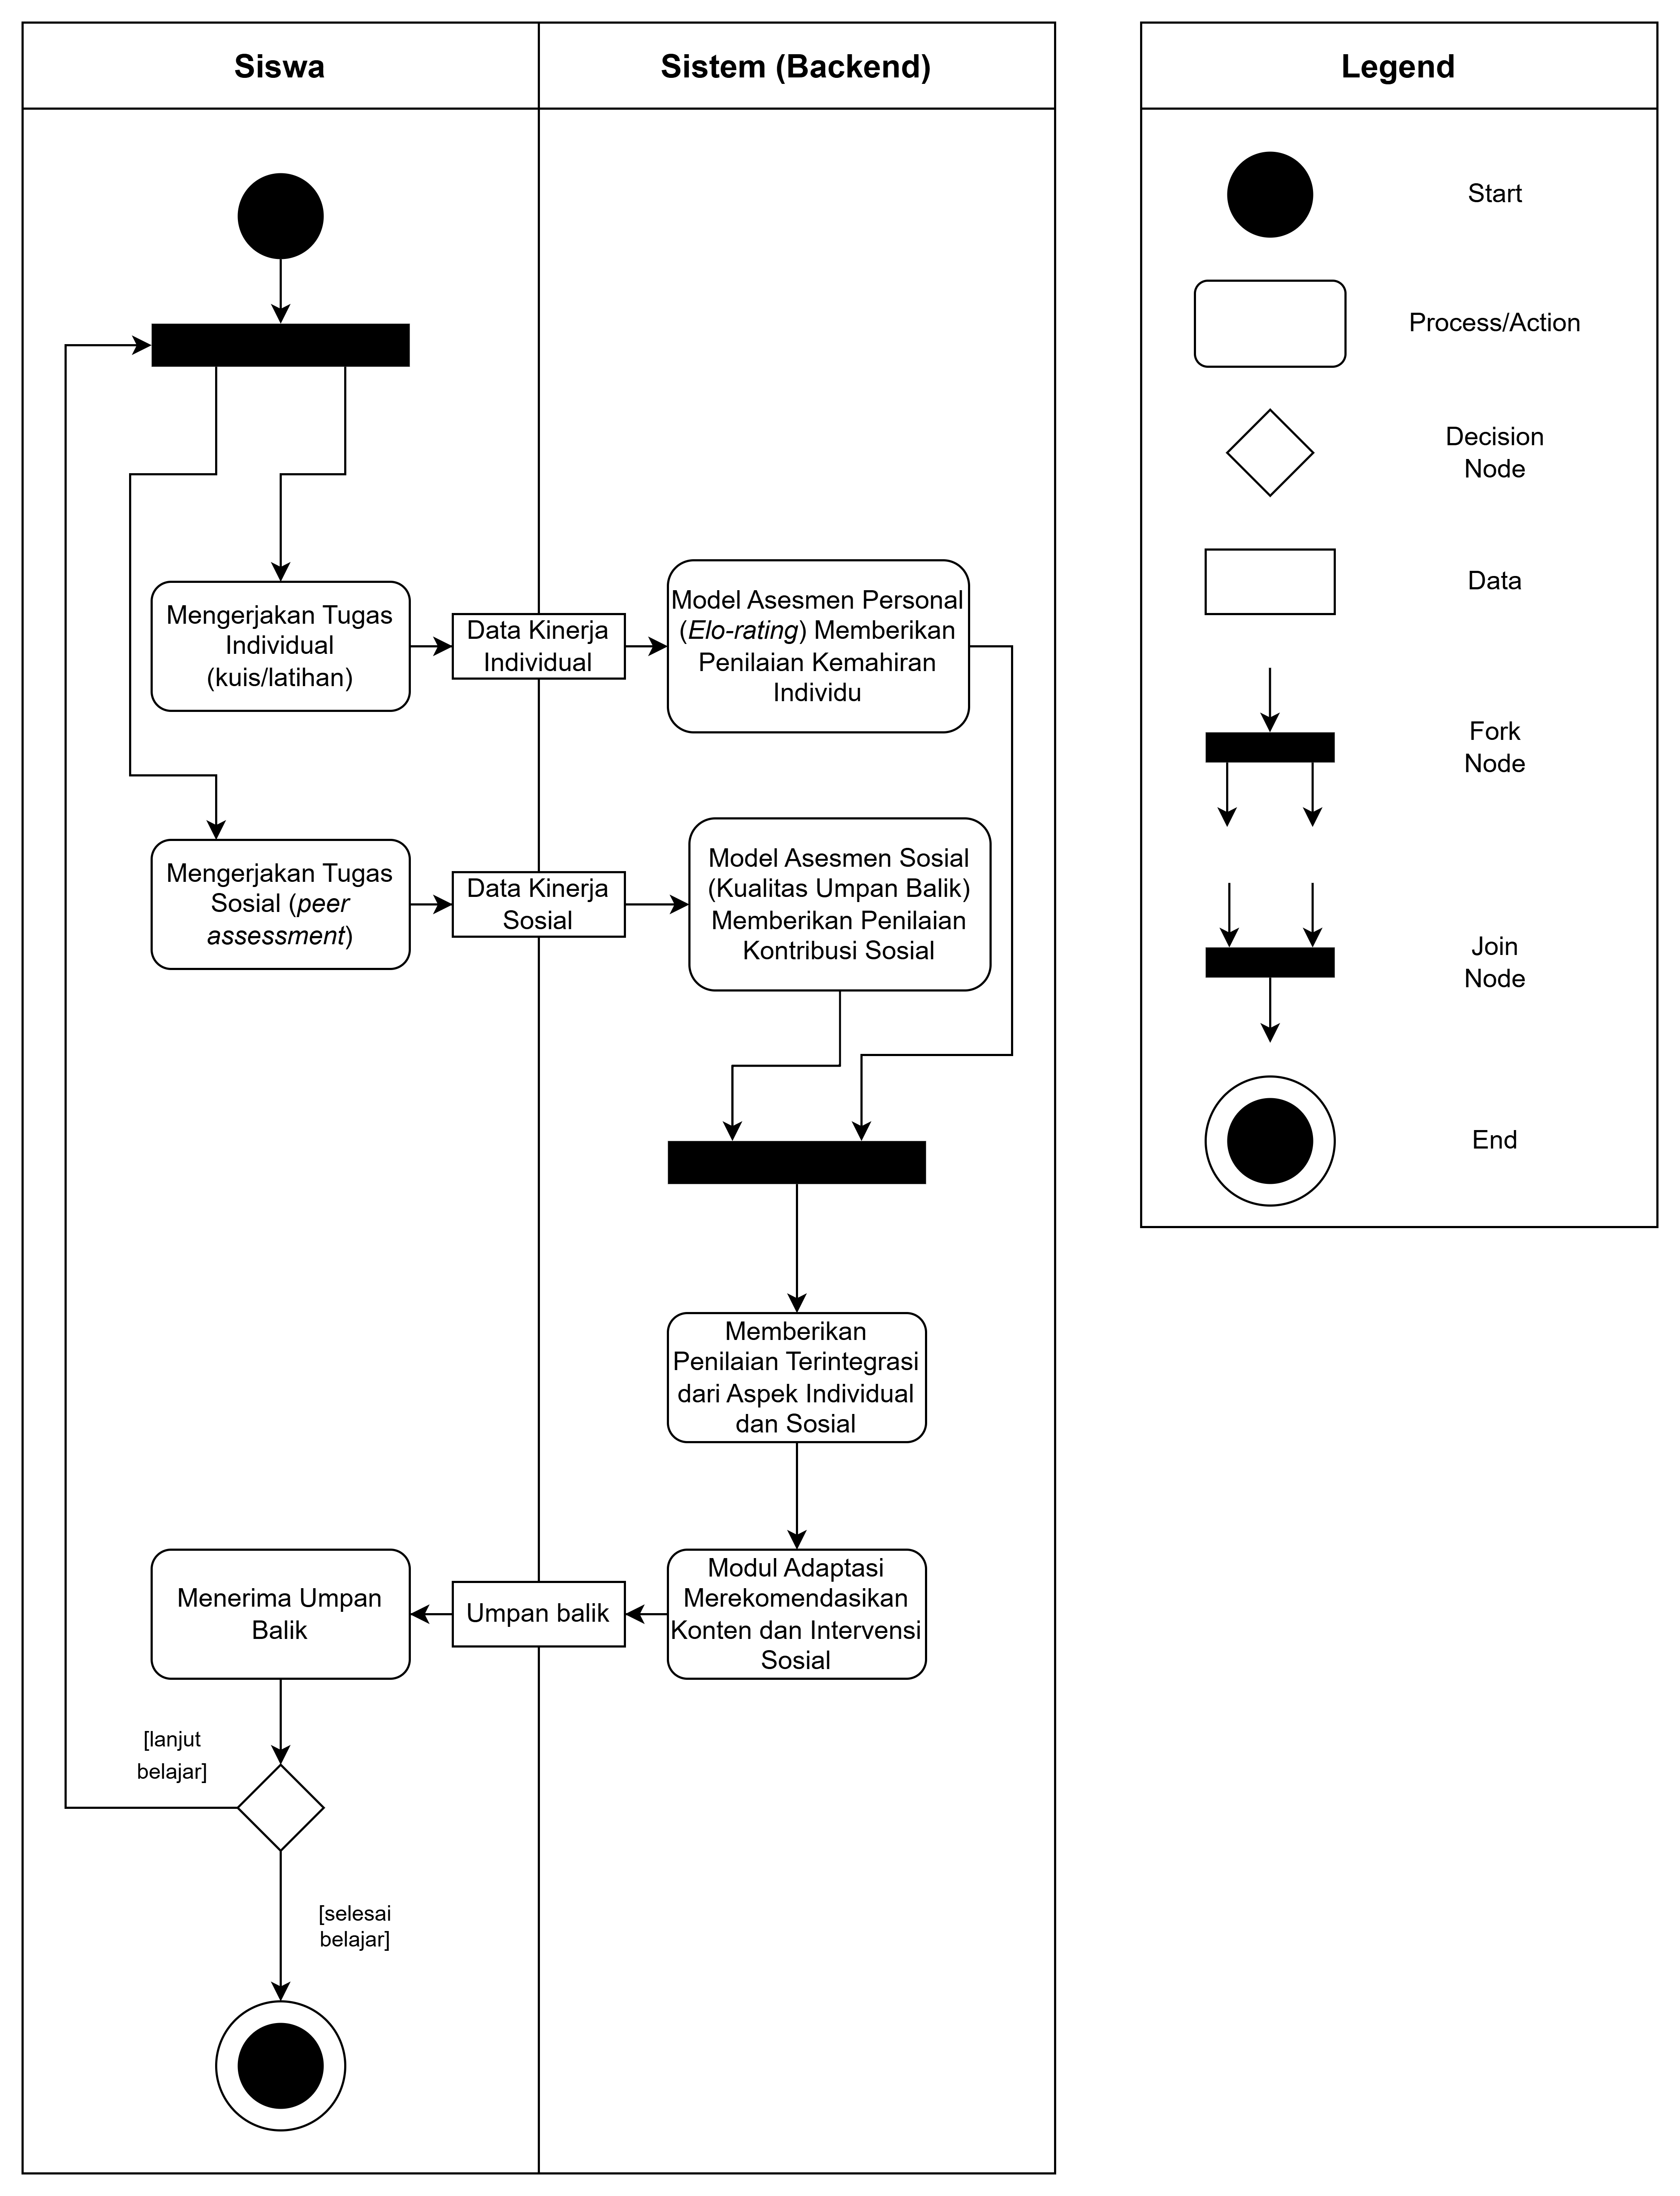
\includegraphics[width=1\textwidth]{image/act_diag_babIV.png} 
    \caption{Model Konseptual Solusi: Arsitektur Integrasi Dinamis (Umpan Balik Ganda) dalam Notasi UML Activity Diagram}
    \label{fig:model-konseptual-solusi}
\end{figure}

% \subsection{Penjelasan Model Konseptual (\textit{After})}
Diagram pada Gambar \ref{fig:model-konseptual-solusi} memodelkan alur kerja solusi yang diusulkan, yang dibagi menjadi dua \textit{swimlanes} (jalur renang) yang merepresentasikan aktor: \textbf{Siswa} (di sisi kiri) dan \textbf{Sistem (Backend)} (di sisi kanan). Alur prosesnya adalah sebagai berikut:

\begin{enumerate}
    \item \textbf{Alur Paralel (Fork):} Setelah proses dimulai (node \textit{Start}), alur kerja langsung memasuki \textit{Fork Node}. Ini mengindikasikan bahwa Siswa dapat mengerjakan dua jenis tugas secara paralel atau dalam urutan yang tidak ditentukan: Tugas Individual dan Tugas Sosial.
    
    \item \textbf{Alur Personal (R1):} 
    \begin{itemize}
        \item \textbf{Aktivitas Siswa:} Siswa \textit{"Mengerjakan Tugas Individual (kuis/latihan)"}.
        \item \textbf{Aliran Data:} Aksi ini menghasilkan \textit{"Data Kinerja Individual"} (misalnya, jawaban benar/salah, waktu pengerjaan).
        \item \textbf{Aktivitas Sistem:} Data ini diterima oleh \textit{backend} dan dieksekusi oleh aktivitas \textbf{"Model Asesmen Personal (Elo-rating) Memberikan Penilaian Kemahiran Individu"}. Aktivitas ini secara spesifik akan dijalankan oleh \textbf{Modul Asesmen Personal} (FR-10) yang telah dipilih. Modul ini memenuhi \textbf{Kebutuhan R1} (Pemodelan Kemahiran Individu) dengan memperbarui skor \textit{Elo-rating} siswa.
    \end{itemize}

    \item \textbf{Alur Sosial (R2 \& R3):}
    \begin{itemize}
        \item \textbf{Aktivitas Siswa:} Siswa \textit{"Mengerjakan Tugas Sosial (peer assessment)"}. Ini memenuhi \textbf{Kebutuhan R2} (Fasilitasi Interaksi Kolaboratif).
        \item \textbf{Aliran Data:} Aksi ini menghasilkan \textit{"Data Kinerja Sosial"} (misalnya, teks umpan balik yang diberikan ke rekan, skor rubrik yang diisi).
        \item \textbf{Aktivitas Sistem:} Data ini diterima oleh \textit{backend} dan dieksekusi oleh aktivitas \textbf{"Model Asesmen Sosial (Kualitas Umpan Balik) Memberikan Penilaian Kontribusi Sosial"}. Aktivitas ini akan dijalankan oleh \textbf{Modul Asesmen Sosial} (FR-11) dan memenuhi \textbf{Kebutuhan R3} (Penilaian Kinerja Kolaboratif), dengan mengukur kualitas umpan balik yang diberikan siswa berdasarkan temuan \textcite{Lu2012}.
    \end{itemize}

    \item \textbf{Integrasi (Join) (R4):}
    \begin{itemize}
        \item \textbf{Aktivitas Sistem:} \textit{Join Node} (garis tebal kedua) menunjukkan bahwa sistem menunggu kedua alur (personal dan sosial) menghasilkan model kemahiran terbaru. Kedua model ini kemudian menjadi \textit{input} untuk aktivitas \textbf{"Memberikan Penilaian Terintegrasi..."}.
        \item \textbf{Modul Pelaksana:} Aktivitas ini dijalankan oleh \textbf{Modul Integrasi Algoritmik} (FR-12). Inilah inti dari solusi yang menjembatani kesenjangan: modul ini secara matematis menggabungkan skor dari Modul Asesmen Personal (Elo) dan Modul Asesmen Sosial (Peer Assess) untuk menciptakan satu Model Kemahiran Holistik. Ini secara langsung memenuhi \textbf{Kebutuhan R4} (Integrasi Model Penilaian).
    \end{itemize}
    
    \item \textbf{Adaptasi (R5):}
    \begin{itemize}
        \item \textbf{Aktivitas Sistem:} Model Kemahiran Holistik yang baru kemudian mengalir ke aktivitas \textbf{"Modul Adaptasi Merekomen..."}.
        \item \textbf{Modul Pelaksana:} Aktivitas ini dijalankan oleh \textbf{Mesin Adaptasi} (FR-13, FR-14). Berdasarkan skor yang terintegrasi, modul ini menghasilkan \textit{"Umpan Balik"} adaptif. Umpan balik ini bisa berupa (a) rekomendasi konten individual, atau (b) intervensi sosial, sehingga memenuhi \textbf{Kebutuhan R5} (Sistem Adaptasi Terintegrasi).
    \end{itemize}

    \item \textbf{Siklus Selesai:} \textit{"Umpan Balik"} dikirimkan kembali ke Siswa, yang \textit{"Menerima Umpan Balik"}. Siswa kemudian dapat memutuskan (\textit{Decision Node}) apakah akan melanjutkan belajar (kembali ke \textit{Fork Node}) atau \textit{"[selesai belajar]"} (menuju node \textit{End}).
\end{enumerate}

\section{Perbandingan (\textit{Before vs After})}
Perbedaan utama antara sistem saat ini (Gambar \ref{fig:model-konseptual-individu} dan \ref{fig:model-konseptual-sosial}) dan solusi yang diusulkan (Gambar \ref{fig:model-konseptual-solusi}) adalah pada sifat integrasinya:

\begin{itemize}
    \item \textbf{\textit{Before} (Sistem Saat Ini):} Integrasi bersifat \textbf{visual} dan \textbf{pasif}. Model personal dan sosial adalah dua entitas terpisah yang hanya ditampilkan berdampingan di antarmuka pengguna (\textit{interface}) \autocite{Brusilovsky2016}.
    \item \textbf{\textit{After} (Solusi yang Diusulkan):} Integrasi bersifat \textbf{algoritmik} dan \textbf{dinamis}. Seperti yang ditunjukkan oleh alur di Gambar \ref{fig:model-konseptual-solusi}, model personal dan sosial adalah dua sumber data yang secara matematis \textbf{digabungkan} di \textit{backend} (pada aktivitas "Memberikan Penilaian Terintegrasi") untuk menciptakan satu model kemahiran holistik yang baru. Model gabungan inilah yang kemudian secara aktif menggerakkan \textit{semua} bentuk adaptasi sistem.
\end{itemize}